There are several image colorization machine learning models available, e.g. - 
\begin{itemize}
    \item GAN
    \item CGAN
    \item DCGAN
    \item Pix2Pix GAN
    \item CycleGAN
    \item Latent Diffusion Model(LDM)
\end{itemize}

But to select the most appropriate image colorization model for our SAR image colorization, we need to look at the features, pros and cons of the available models and decide which model's features aligns with our goals the best.

\section*{GAN}
GANs (Generative Adversarial Network) are a class of neural networks that autonomously learn patterns in the input data to generate new samples resembling the original dataset.
GAN's architecture consists of two neural networks:\par
    \textbf{\textit{Generator} -} Creates synthetic data from random noise to produce data so realistic that the discriminator cannot distinguish it from real data.\par
    \textbf{\textit{discriminator} -} Acts as a critic, evaluating whether the data it receives is real or fake.

\section*{CGAN}
A Conditional Generative Adversarial Network (CGAN) is an advanced type of GAN (Generative Adversarial Network) where output generation is controlled using a condition.\par
For example, if you want to generate only Mercedes cars from a dataset of various cars, CGANs allow you to specify "Mercedes" as a condition.

\section*{DCGAN}
DCGAN, ot Deep Convolutional Generative Adversarial Network uses a generator composed of a series of transpose convolution operations. These operations take in a random noise vector, z, and transform it by progressively increasing its spatial dimensions while decreasing its feature volume depth. The discriminator is basically a convolutional neural network which classifies an image as real or fake.

\section*{Pix2Pix GAN}
It uses CGAN model and U-net architecture to perform image-to-image translations. But we can only provide images as input, no text can be provided as input prompt.

\section*{CycleGAN}
In CycleGAN, we treat the problem as an image reconstruction problem. We first take an image input (x) and use the generator G to convert it into the transformed image. Then we reverse this process from transformed image to original image using a generator F. Then we calculate the mean squared error loss between real and reconstructed image.\par
The most important feature of this cycle GAN is that it can do this image translation on an unpaired image where there is no relation exists between the input image and output image.

\section*{Latent Diffusion Model}
The key innovation of latent diffusion models is that they apply this diffusion process not to the raw pixel values of an image but instead to an encoded latent representation of the image.
How it Works:
\begin{itemize}
    \item \textbf{Encoding:} An input image is encoded by the autoencoder into a latent representation. 
    \item \textbf{Forward Diffusion:} The latent representation is progressively corrupted by adding noise. 
    \item \textbf{Reverse Diffusion:} The denoising U-Net iteratively removes the noise from the corrupted latent representation, guided by the conditioning input (e.g., text). 
    \item \textbf{Decoding:} The denoised latent representation is decoded by the autoencoder to produce the final generated image.
\end{itemize}

\section{Why latent diffusion model?} \label{sec:WhyLDM}

\textbf{Our Objective :} To train the model with paired images(black-and-white images and their corresponding colored images) and a text prompt, so that we can provide the model any new black-and-white image and get the corresponding colorized image.
\par A comparison chart of the previously discussed image colorization models is given below -

\begin{table}[h!]
\centering
\begin{tabular}{|l|c|c|c|c|c|}
\hline
\textbf{Model} & \textbf{Prompt Input} & \textbf{Image Quality} & \textbf{Required Paired Data} & \textbf{Stability} & \textbf{Control} \\
\hline
GAN & No & High & No & No & No \\
CGAN & Yes & High & Yes & No & Yes \\
DCGAN & No & Moderate & No & No & No \\
Pix2Pix GAN & Yes (Image) & Very High & Yes & Yes & Yes \\
CycleGAN & No & Moderate & No & Yes & No \\
LDM & Yes (Text/Image) & Very High & Yes & Yes & Yes \\
\hline
\end{tabular}
\caption{Comparison of deep generative models for SAR image colorization}
\label{tab:model_comparison}
\end{table}

As shown in Table~\ref{tab:model_comparison}, LDM offers the highest control, stability and image quality. It also supports text/image prompt input and training using paired data - which clearly satisfies our objective for SAR image colorization.\par
Also, by operating in this compressed latent space instead of directly on pixels, latent diffusion model offers several key advantages:
\begin{itemize}
    \item \textbf{Computationally efficient:} The smaller latent space representation makes executing the diffusion process much faster. This allows the models to be trained on consumer GPUs rather than requiring hundreds of GPUs like pixel-based diffusion models.
    \item \textbf{High resolution:} The decoder upsamples the modified latent code into a high-resolution output image, enabling manipulation of images at resolutions not possible with raw pixels.
    \item \textbf{Flexible conditioning:} Text, images, segmentation maps and other inputs can be encoded into the latent space and used to condition the model to generate outputs with desired characteristics.
    \item \textbf{Detail preservation:} The encoder-decoder structure allows for manipulating images while still preserving intricate details from the original inputs.
\end{itemize}

Hence, Latent Diffusion Model is the most suitable and appropriate choice for our project. 

\section{Components of LDM}


The Latent Diffusion Model (LDM) is a type of generative model that operates in a compressed latent space, making it both computationally efficient and capable of producing high-quality outputs. The architecture of an LDM typically integrates the following three major components:

\subsection*{1. Variational Autoencoder (VAE)}
The VAE is responsible for mapping high-dimensional image data to a lower-dimensional latent space. It consists of an encoder that compresses the input image into a latent representation and a decoder that reconstructs the image from the latent code. By training the VAE to preserve the most important semantic and structural features, the diffusion process can be applied in the latent space instead of the pixel space, significantly reducing computational overhead.

\subsection*{2. Contrastive Language-Image Pretraining (CLIP)}
CLIP is a vision-language model that learns a shared embedding space for images and text. In the context of LDMs, CLIP can be used for conditional generation by incorporating text-based prompts or semantic guidance during training or inference. This allows the model to generate images that are not only visually plausible but also aligned with high-level descriptions or attributes, which can be extended to the SAR colorisation task in future work.

\subsection*{3. U-Net Architecture}
The U-Net serves as the core neural network used in the denoising process of the diffusion model. It takes a noisy latent representation as input and predicts the noise to be removed at each diffusion step. The U-Net used in LDMs is often enhanced with attention mechanisms and conditional embeddings (e.g., timestep embeddings, CLIP embeddings) to improve the generative capabilities. Its symmetric encoder-decoder structure with skip connections helps preserve spatial details across the layers.

Together, these components enable the LDM to learn efficient, controllable, and high-fidelity mappings from noisy latent variables to clean, semantically rich images.


\subsection{VAE}

\subsubsection{What is a Variational Autoencoder (VAE)?}
A Variational Autoencoder, or VAE, is a type of generative model that learns both how to represent data in a compressed form (encoding) and how to reconstruct data from that compressed form (decoding). Unlike traditional autoencoders, VAEs introduce a probabilistic element, allowing them to learn meaningful latent representations of data. This makes them useful for tasks like image generation, representation learning, and semi-supervised learning.

\subsubsection{Architecture and Working Mechanism}
VAEs consist of two major parts:
\begin{itemize}
    \item \textbf{Encoder (Inference Model):} Transforms input data into a lower-dimensional latent space, where each data point is represented as a probability distribution rather than a single point. This is typically modeled using a neural network that outputs the parameters of a Gaussian distribution (mean and variance).
    \item \textbf{Decoder (Generative Model):} Reconstructs the original data from a sample drawn from the latent distribution. This helps the model generate new data that resembles the input space.
\end{itemize}

To make learning efficient, VAEs use a technique called the \textit{reparameterization trick} \cite{Kingma_2019}, which enables gradients to flow through stochastic nodes during backpropagation. This trick transforms the sampling operation into a deterministic function plus random noise, making it compatible with gradient-based optimization methods.

\subsubsection{Optimization: The ELBO}
The VAE does not optimize the likelihood of the data directly. Instead, it uses a surrogate objective called the Evidence Lower Bound (ELBO), which balances two terms:
\begin{itemize}
    \item A reconstruction term, which ensures the decoded output is similar to the input.
    \item A regularization term (KL divergence), which ensures the learned latent space follows a standard normal distribution.
\end{itemize}
Maximizing the ELBO allows the model to learn both how to compress data and how to generate new samples effectively.

\subsubsection{Features and Capabilities}
\begin{itemize}
    \item \textbf{Latent Space Modeling:} Learns structured and interpretable latent variables.
    \item \textbf{Generative Abilities:} Can create new samples by drawing from the latent distribution.
    \item \textbf{Amortized Inference:} The encoder is shared across all inputs, making inference faster and more scalable.
    \item \textbf{Smooth Interpolations:} Because of the probabilistic nature of the latent space, interpolating between two points results in smooth transitions in the generated output.
\end{itemize}

\subsubsection{Comparison with Other Models}
Unlike GANs, which focus on generating sharp, realistic outputs without explicitly modeling the data distribution, VAEs aim to model the full data distribution and offer better control and interpretability over the latent space. While they sometimes produce blurrier outputs, VAEs excel at representing uncertainty and allow easy sampling, interpolation, and conditional generation.

\subsubsection{Why Use VAE?}
In our SAR image colorization setup, we need a system that can handle paired grayscale and color images and learn to represent their relationship in a structured way. The VAE’s probabilistic framework and ability to model high-dimensional distributions through a compressed latent space make it a strong candidate for this task \cite{Kingma_2019}. Its compatibility with other components like UNET (as a decoder) and CLIP (for prompt-based conditioning) makes it especially suitable for our multimodal image-to-image translation pipeline.


\subsection{CLIP}

\subsubsection{What is CLIP?}
Contrastive Language–Image Pretraining (CLIP) is a neural network model introduced by OpenAI that learns to connect images and text by training on a massive dataset of 400 million (image, text) pairs collected from the internet \cite{radford2021learningtransferablevisualmodels}. Unlike traditional supervised models that rely on task-specific labeled data, CLIP is trained with natural language supervision using a contrastive learning objective. Its dual-encoder structure includes both an image encoder and a text encoder, enabling CLIP to perform zero-shot transfer across a variety of vision tasks.

\subsubsection{Architecture of the Text Encoder}
The CLIP text encoder is a transformer-based architecture similar in design to GPT-2 \cite{radford2021learningtransferablevisualmodels}. It operates on a byte pair encoded (BPE) tokenized input with positional embeddings and uses masked self-attention. The encoded text is projected into a joint embedding space shared with image embeddings. Specifically, the final layer's output corresponding to the \texttt{[EOS]} token is extracted and linearly projected for contrastive learning alignment.

\subsubsection{Working Mechanism}
During training, CLIP is optimized to distinguish correct (image, text) pairs from incorrect ones using a symmetric InfoNCE loss. Given a batch of $N$ (image, text) pairs, the model learns embeddings such that the cosine similarity between matched pairs is maximized, and mismatches are minimized. This is done for both directions: image-to-text and text-to-image.

\subsubsection{Features and Capabilities}
\begin{itemize}
    \item \textbf{Zero-shot Learning}: CLIP performs tasks without any additional fine-tuning, simply by using textual prompts.
    \item \textbf{Flexible Prompting}: Users can guide CLIP with different natural language phrases, allowing contextual control over predictions.
    \item \textbf{Text Encoder for NLP}: Although trained for vision-language tasks, the CLIP text encoder can be repurposed for phrase understanding and even outperforms traditional language models like BERT in certain tasks \cite{yan2022clipunderstandstextprompting}.
    \item \textbf{Open-vocabulary Classification}: Since labels are given as text, CLIP can recognize classes it has never seen during training.
\end{itemize}

\subsubsection{Comparison with Other Models}
Unlike BERT, which uses masked language modeling, or GPT, which uses autoregressive prediction, CLIP uses a contrastive loss across modalities. This enables alignment between vision and language but limits the encoder's performance on typical NLP tasks unless prompted appropriately. Nonetheless, when evaluated on phrase understanding and entity tasks, CLIP often outperforms BERT and other specialized models \cite{yan2022clipunderstandstextprompting}.

\subsubsection{Why Use CLIP?}
CLIP excels in:
\begin{itemize}
    \item \textbf{Cross-modal understanding}, bridging visual and textual inputs.
    \item \textbf{Zero-shot generalization}, enabling use without task-specific data.
    \item \textbf{Scalability and flexibility}, through prompt engineering and contrastive training.
    \item \textbf{Compact design}, with a 38M parameter text encoder that performs competitively against much larger models \cite{yan2022clipunderstandstextprompting}.
\end{itemize}

In SAR image colorization, where we take black-and-white satellite images as input paired with a label (text prompt) to generate the corresponding colorized image, the ability to robustly understand and align textual descriptions with visual content is crucial. The CLIP text encoder provides an effective solution by mapping input prompts into a shared embedding space with images, enabling models to accurately associate textual labels with visual features. This makes it an excellent choice for text-to-image generation and conditioning tasks, particularly in remote sensing domains where annotation is limited and interpretability is key. With its scalable training strategy, strong generalization, and lightweight architecture, CLIP offers a compelling foundation for multimodal SAR-based applications.



\subsection{UNET}

\subsubsection{What is UNET?}
UNET is a type of convolutional neural network developed specifically for image segmentation tasks in the biomedical field. It was designed to deliver high accuracy using only a small amount of labeled data. The model's structure forms a distinctive U-shape, which allows it to combine detailed spatial information with broader contextual features. This makes UNET especially effective for applications where both fine detail and global structure are important.

\subsubsection{Architecture}
The network has two main sections:
\begin{itemize}
    \item \textbf{Contracting Path:} This section works like a typical convolutional neural network. It repeatedly applies small filters and pooling to reduce the size of the feature maps while increasing the number of channels. This helps the network capture more abstract features as the image size shrinks.
    \item \textbf{Expanding Path:} In this phase, the network gradually increases the resolution by upsampling. It also connects features from earlier layers in the contracting path, allowing the model to recover fine spatial details lost during downsampling.
\end{itemize}
This U-shaped design enables the model to consider both local and global image contexts, producing accurate segmentations.\cite{ronneberger2015unetconvolutionalnetworksbiomedical}

\subsubsection{Working Mechanism}
UNET works by classifying each pixel in an image. It uses a softmax function \cite{ronneberger2015unetconvolutionalnetworksbiomedical} to assign probabilities to different classes, and a loss function that compares the predictions to the true pixel labels. To handle imbalanced data and emphasize important regions (such as boundaries between objects), the loss function includes a weight map.

Additionally, the model uses a technique called \textit{overlap-tile strategy} to process large images. When the input image exceeds the model's capacity, it's divided into overlapping tiles. Border areas are filled using mirroring to ensure smooth predictions at the edges.

\subsubsection{Features and Capabilities}
\begin{itemize}
    \item \textbf{Detailed segmentation:} It accurately labels each pixel by combining low- and high-level image features.
    \item \textbf{Efficient with small datasets:} The model can be trained with limited annotated data using extensive data augmentation, such as elastic distortions.
    \item \textbf{Quick and scalable:} It can process standard-size images (e.g., 512×512 pixels) in under a second on modern hardware.
    \item \textbf{Adaptable to large images:} Through the overlap-tile strategy, it can handle inputs of any size.
\end{itemize}

\subsubsection{Comparison with Other Models}
Unlike earlier models that slide a window over the image to make predictions, UNET processes the full image at once. This speeds up prediction and improves accuracy by avoiding redundant computations. Compared to simpler CNNs, UNET’s skip connections help preserve fine image details that are often lost in deeper networks.

\subsubsection{Why Use UNET?}
UNET is a solid choice for tasks that require high-resolution outputs, especially where detailed structure needs to be preserved—such as in SAR image colorization. Its ability to work well with limited training data and retain intricate features in the output makes it a reliable component when paired with models like Latent Diffusion.In our project, UNET plays a vital role in the decoder part of the pipeline, helping generate precise, realistic colorizations from SAR grayscale images.


\section{Architecture Overview}

Our approach utilizes a two-stage generative model for SAR to optical image translation:

\begin{enumerate}
    \item \textbf{Stage 1}: Variational Autoencoder (VAE) learns a compact latent representation of optical images
    \item \textbf{Stage 2}: Conditional diffusion model generates optical latents from SAR inputs with text guidance
\end{enumerate}

\subsection{System Architecture}

The overall system architecture can be visualized as follows:

\begin{center}
\texttt{SAR Image (256×256×3)} $\rightarrow$ \\
\texttt{VAE Encoder} $\rightarrow$ \texttt{Latents (64×64×4)} $\rightarrow$ \\
\texttt{U-Net} $\rightarrow$ \texttt{Enhanced Latents (64×64×4)} $\rightarrow$ \\
\texttt{VAE Decoder} $\rightarrow$ \texttt{Optical Image (256×256×3)} \\
$\uparrow$ \\
\texttt{Text Prompt}
\end{center}

\subsection{Model Components}

\subsubsection{Variational Autoencoder (VAE)}

\textbf{Purpose}: Learns a discrete latent representation space for optical images.

\textbf{Architecture Components}:

\textbf{Encoder}:
\begin{itemize}
    \item Input: RGB optical images (256×256×3)
    \item Convolutional layers with progressive downsampling
    \item Down channels: [64, 128, 256, 256]
    \item Downsampling stages: 3 (256→128→64→32, then upsampled to 64×64)
    \item Output: Continuous latents (64×64×4)
\end{itemize}

\textbf{Decoder}:
\begin{itemize}
    \item Input: Quantized latents (64×64×4)
    \item Progressive upsampling to original resolution
    \item Output: Reconstructed RGB images (256×256×3)
\end{itemize}

\subsubsection{U-Net Diffusion Model}

\textbf{Purpose}: Generates optical image latents conditioned on SAR images and text prompts using denoising diffusion.

\textbf{Architecture Specifications}:
\begin{itemize}
    \item \textbf{Backbone}: U-Net with skip connections
    \item \textbf{Down channels}: [256, 384, 512, 768]
    \item \textbf{Mid channels}: [768, 512]
    \item \textbf{Attention mechanisms}: Multi-head self-attention at each resolution level
\end{itemize}

\textbf{Conditioning Mechanisms}:

\begin{enumerate}
    \item \textbf{SAR Image Conditioning}:
    \begin{itemize}
        \item Direct spatial feature concatenation
        \item Cross-attention integration in U-Net blocks
        \item Dropout probability: 5\% (for classifier-free guidance)
    \end{itemize}
    
    \item \textbf{Text Conditioning}:
    \begin{itemize}
        \item CLIP text encoder
        \item Embedding dimension: 512
        \item Cross-attention integration
        \item Dropout probability: 10\% (for classifier-free guidance)
    \end{itemize}
\end{enumerate}

\textbf{Diffusion Process}:

Forward process (noise addition):
\begin{equation}
q(x_t|x_{t-1}) = \mathcal{N}(x_t; \sqrt{1-\beta_t}x_{t-1}, \beta_t I)
\end{equation}

Reverse process (denoising):
\begin{equation}
p_\theta(x_{t-1}|x_t, c) = \mathcal{N}(x_{t-1}; \mu_\theta(x_t, t, c), \Sigma_\theta(x_t, t, c))
\end{equation}

Where $c$ represents the conditioning information (SAR image + text).

\section{Training Methodology}

\subsection{Two-Stage Training Protocol}

\subsubsection{Stage 1: VAE Training}

\textbf{Dataset}: Optical images from Sentinel-2 satellite data

\textbf{Training Configuration}:
\begin{itemize}
    \item Epochs: 25
    \item Batch size: 8
    \item Learning rate: $1 \times 10^{-5}$
    \item Optimizer: Adam
    \item Gradient accumulation: 4 steps
\end{itemize}

\textbf{Loss Function}:
\begin{equation}
\mathcal{L}_{total} = \mathcal{L}_{MSE} + \mathcal{L}_{codebook} + 0.2 \times \mathcal{L}_{commitment} + 0.5 \times \mathcal{L}_{adversarial}
\end{equation}

\subsubsection{Stage 2: Latent Diffusion Model Training}

\textbf{Dataset}: SAR-optical image pairs with text descriptions

\textbf{Training Configuration}:
\begin{itemize}
    \item Epochs: 60
    \item Batch size: 16
    \item Learning rate: $1 \times 10^{-4}$
    \item Optimizer: Adam
    \item Diffusion timesteps: 1,000
    \item Beta schedule: Linear (0.00085 → 0.012)
\end{itemize}

\textbf{Training Process}:
\begin{enumerate}
    \item \textbf{Latent Encoding}: Optical images encoded to latents using trained VQ-VAE
    \item \textbf{Noise Addition}: Random timestep $t$ sampled, noise added to latents
    \item \textbf{Conditional Prediction}: U-Net predicts noise given noisy latents and conditions
    \item \textbf{Loss Computation}: MSE between predicted and actual noise
\end{enumerate}

\textbf{Noise Prediction Objective}:
\begin{equation}
\mathcal{L}_{diffusion} = \mathbb{E}_{t,\epsilon \sim \mathcal{N}(0,I),c} \left[ \|\epsilon - \epsilon_\theta(\sqrt{\bar{\alpha}_t}x_0 + \sqrt{1-\bar{\alpha}_t}\epsilon, t, c)\|^2 \right]
\end{equation}

\subsection{Data Configuration}

\textbf{Dataset Splits}:
\begin{itemize}
    \item Training: 70\%
    \item Validation: 15\%
    \item Testing: 15\%
\end{itemize}

\textbf{Data Augmentation}:
\begin{itemize}
    \item Geometric transformations (rotation, flipping)
    \item Color jittering for optical images
\end{itemize}

\textbf{Text Prompt Format}:
\begin{center}
\texttt{"Colorise image, Region: \{region\}, Season: \{season\}"}
\end{center}

Where:
\begin{itemize}
    \item \texttt{region}: \{tropical, temperate, arctic\}
    \item \texttt{season}: \{spring, summer, autumn, winter\}
\end{itemize}

\subsection{Implementation Details}

\textbf{Hardware Requirements}:
\begin{itemize}
    \item GPU: NVIDIA H200 140GB (104 GB in use during training)
    \item RAM: 50 GB
    \item Storage: 50GB
\end{itemize}

\textbf{Training Performance}:
\begin{itemize}
    \item VAE training time: 10 minutes per epoch
    \item LDM training time: 6 minutes per epoch
    \item Total training time: 13 hours
\end{itemize}

\begin{figure}[h!]
    \centering
    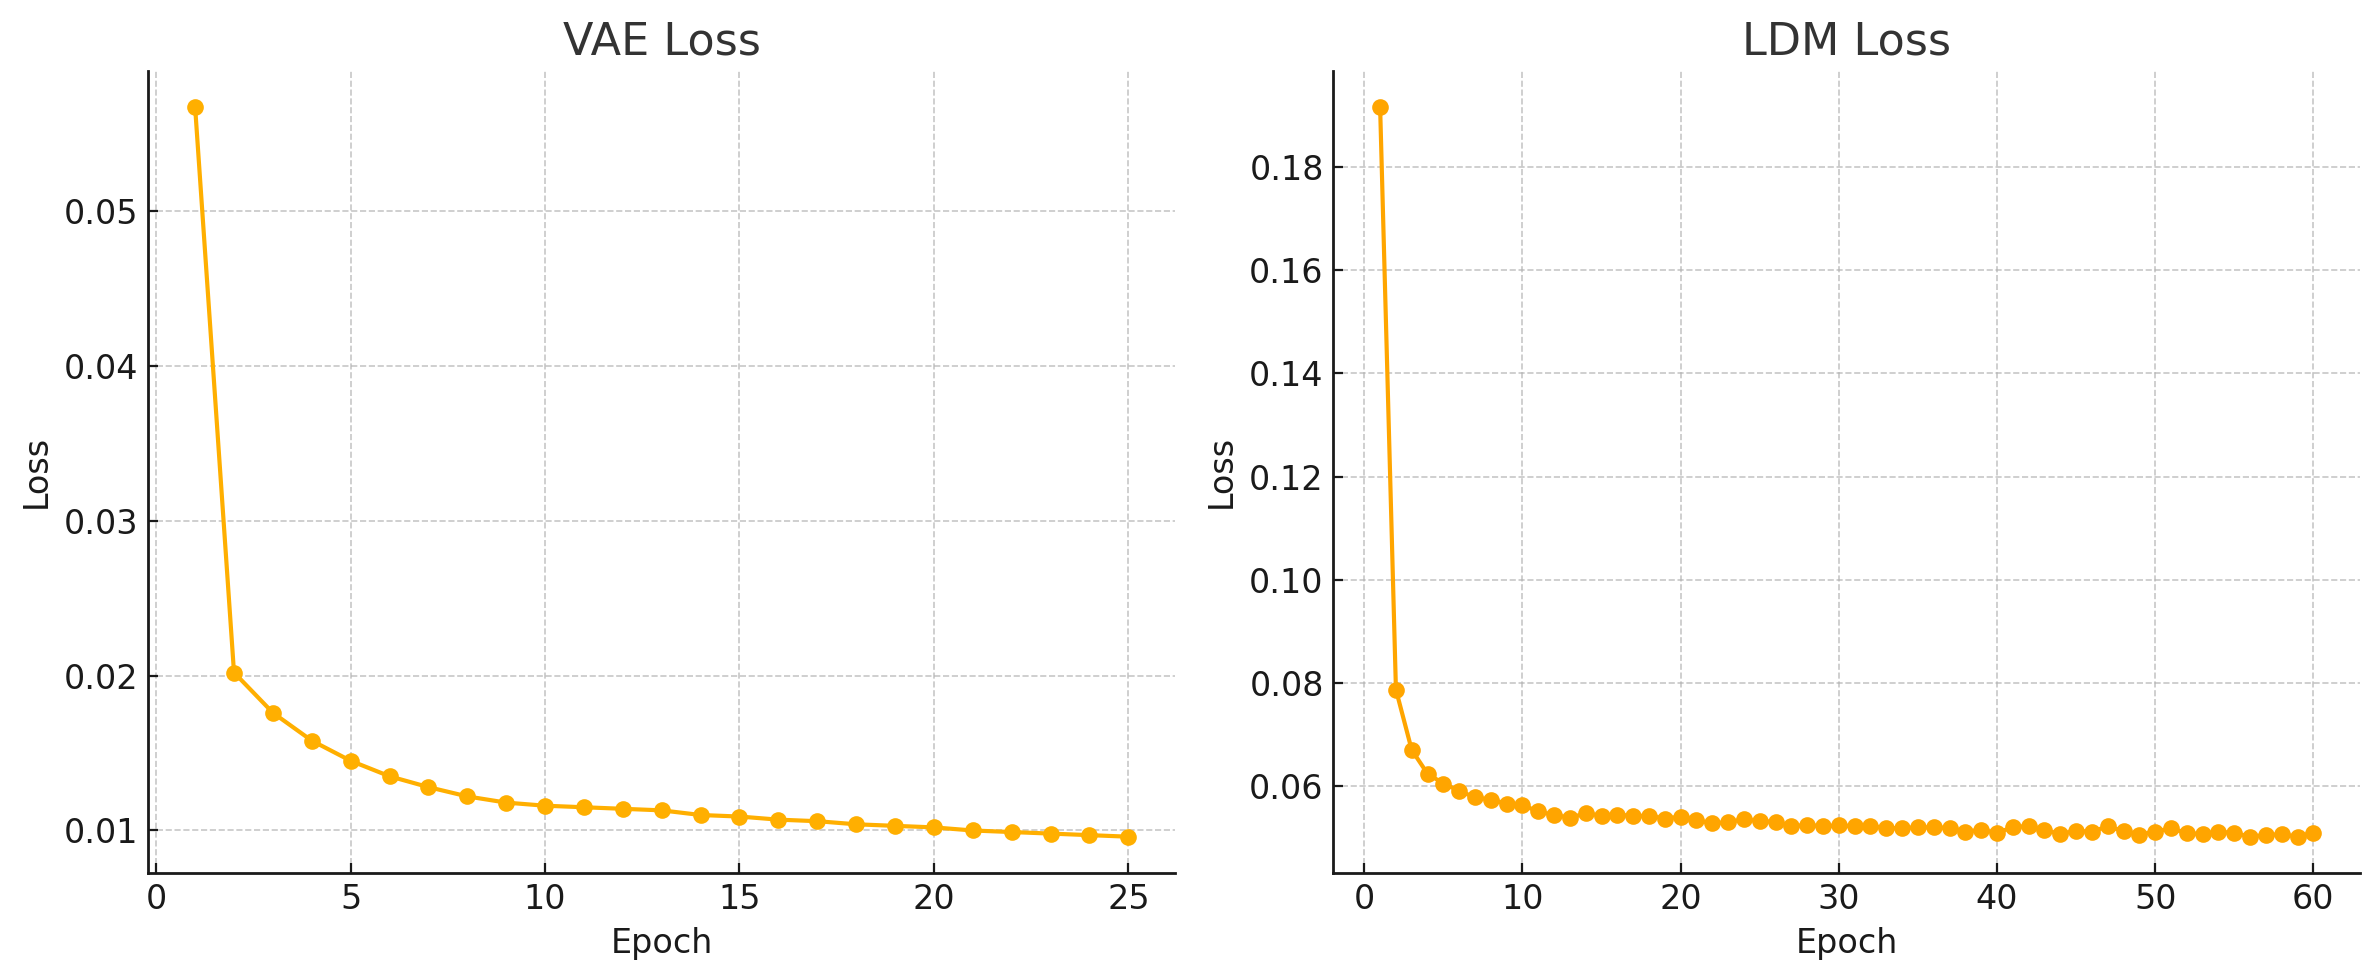
\includegraphics[width=0.8\textwidth]{loss_curve.png}
    \caption{Training loss curves for both VAE and LDM training stages}
    \label{fig:loss_curve}
\end{figure}